\let\negmedspace\undefined
\let\negthickspace\undefined
\documentclass[journal]{IEEEtran}
\usepackage[a5paper, margin=10mm, onecolumn]{geometry}
\usepackage{lmodern} % Ensure lmodern is loaded for pdflatex
\usepackage{tfrupee} % Include tfrupee package

\setlength{\headheight}{1cm} % Set the height of the header box
\setlength{\headsep}{0mm}     % Set the distance between the header box and the top of the text

\usepackage{gvv-book}
\usepackage{gvv}
\usepackage{cite}
\usepackage{amsmath,amssymb,amsfonts,amsthm}
\usepackage{algorithmic}
\usepackage{graphicx}
\graphicspath{{./figs/}}
\usepackage{textcomp}
\usepackage{xcolor}
\usepackage{txfonts}
\usepackage{listings}
\usepackage{enumitem}
\usepackage{mathtools}
\usepackage{gensymb}
\usepackage{comment}
\usepackage[breaklinks=true]{hyperref}
\usepackage{tkz-euclide} 
\usepackage{listings}
\usepackage{gvv}                                        
\def\inputGnumericTable{}                                 
\usepackage[latin1]{inputenc}                                
\usepackage{color}                                            
\usepackage{array}                                            
\usepackage{longtable}                                       
\usepackage{calc}                                             
\usepackage{multirow}                                         
\usepackage{hhline}                                           
\usepackage{ifthen}                                           
\usepackage{lscape}
\usepackage{circuitikz}
\tikzstyle{block} = [rectangle, draw, fill=blue!20, 
text width=4em, text centered, rounded corners, minimum height=3em]
\tikzstyle{sum} = [draw, fill=blue!10, circle, minimum size=1cm, node distance=1.5cm]
\tikzstyle{input} = [coordinate]
\tikzstyle{output} = [coordinate]
\begin{document}
\bibliographystyle{IEEEtran}
\vspace{3cm}
\title{2.9.1}
\author{EE25BTECH11050-Hema Havil}
\maketitle
	% \newpage
	% \bigskip
	{\let\newpage\relax\maketitle}
	
	\renewcommand{\thefigure}{\theenumi}
	\renewcommand{\thetable}{\theenumi}
	\setlength{\intextsep}{12pt} % Space between text and floats
	
	\numberwithin{equation}{enumi}
	\numberwithin{figure}{enumi}
	\renewcommand{\thetable}{\theenumi}
	
	\textbf{Question}:\\
        Jagdish has a field which is in the shape of a right-angled triangle AQC. He wants to leave a space in the form of a square PQRS inside the field for growing wheat and the remaining space for growing vegetables. In the field, there is a pole marked as O. Based on the above information, answer the following equations
        \begin{enumerate}[label=\alph*)]
            \item Taking O as the origin, P = (-200, 0) and Q = (200, 0). PQRS being a square, what are the coordinates of R and S?
            \item 
            \begin{enumerate}[label=\roman*)]
                \item What is the area of square PQRS ?
                \item What is the length of diagonal PR in PQRS ?
            \end{enumerate}
            \item If S divides CA in the ratio K : 1, what is the value of K, where A = (200, 800)?
        \end{enumerate}
        \solution \\
        Given that,\\ AQC is a right angled triangle at point Q and PQRS is a square inside the $\Delta$AQC, 
        \begin{enumerate}[label=(\alph*)]
            \item We were given two points 
            \begin{align}
                P=(-200,0),Q=(200,0)
            \end{align}
            Let,\\ X be the vector along the side PQ,\\ Y be the vector along the side QR,\\Z be the vector along the side PS then, \\
            \begin{align}
                \vec{X}=\vec{Q}-\vec{P}=\myvec{200\\0}-\myvec{-200\\0}
            \end{align}
            \begin{align}
                \vec{X}=\myvec{400\\0}
            \end{align}
            Rotation vector for 2x2 matrix is 
            \begin{align}
                \vec{R_\theta}=\myvec{cos \theta \; -sin \theta\\sin \theta\;\;\;cos \theta}
            \end{align}
            Rotate the vector $\vec{X}$ by $90^{\circ}$ anticlockwise to get Y
            \begin{align}
                \vec{Y}=\vec{R_{90}}\vec{X}
            \end{align}
            \begin{align}
                \vec{Y}=\myvec{0\;-1\\1\;\;\;\;0}\myvec{400\\0}
            \end{align}
            \begin{align}
                \vec{Y}=\myvec{0\\400}
            \end{align}
            So the vector along the side QR is $\vec{Y}=\myvec{0\\400}$ then,
            \begin{align}
                \vec{Y}=\vec{R}-\vec{Q}
            \end{align}
            \begin{align}
                \vec{R}=\vec{Y}+\vec{Q}
            \end{align}
            \begin{align}
                \vec{R}=\myvec{0\\400}+\myvec{200\\0}
            \end{align}
            \begin{align}
                \vec{R}=\myvec{200\\400}
            \end{align}
            Since the sides QR and PS are parallel, vectors $\vec{Y}=\vec{Z}$ then
            \begin{align}
                \vec{Z}=\vec{S}-\vec{P}
            \end{align}
            \begin{align}
                \vec{S}=\vec{Z}+\vec{P}
            \end{align}
            \begin{align}
                \vec{S}=\myvec{0\\400}+\myvec{-200\\0}
            \end{align}
            \begin{align}
                \vec{S}=\myvec{-200\\400}
            \end{align}
            Therefore the coordinates of the points R and S are (200,400) and (-200,400)
            \item
            \begin{enumerate}[label=(\roman*)]
                \item We know the points P(-200,0) and Q(200,0)\\
                   Let length of the side of the square PQRS be x then,
                   \begin{align}
                       x=\norm{\vec{Q}-\vec{P}}
                   \end{align}
                   \begin{align}
                       x=\norm{\myvec{400\\0}}=400
                   \end{align}\\
                
                Area of the square = $x^2$ = $(400)^2$ = 160000 sq units\\
                \item Length of diagnol of the square = $x\sqrt{2}$ = $400\sqrt{2}$ units\\
            \end{enumerate}
            \item Given the point A=(200,800)\\
            Since it was given that point S divides CA in the ratio K:1, this shows that points A,C and S are collinear. Since AQC is a right angled triangle, from this we can say that point C lies on X axis\\
            Let point C be (t,0), Consider the matrix M\\
            \begin{align}
                M = \myvec{x_1\;\;y_1\;\;1\\x_2\;\;y_2\;\;1\\x_3\;\;y_3\;\;1}
            \end{align}
            Where the points in the matrix are A(200,800),S(-200,400) and C(t,0) then,\\ substitute in ((c).1)
            \begin{align}
                M = \myvec{200\;800\;\;1\\-200\;400\;1\\t\;\;\;\;\;0\;\;\;\;\;\;1}
            \end{align}
            For the points to be collinear rank of matrix M should be equal to 2,\\
            By applying row transformations,\\\\
            {\large$R_1\rightarrow{}\frac{1}{200}R_1$}
            \begin{align}
                 M = \myvec{1\;\;\;\;\;\;4\;\;\;\;\;\frac{1}{200}\\-200\;400\;1\\t\;\;\;\;\;0\;\;\;\;\;\;1}
            \end{align}
            {\large$R_2\rightarrow{}R_2 + 200R_1$}\hspace{2cm}
            {\large$R_3\rightarrow{R_3 - tR_1}$}
            \begin{align}
                 M = \myvec{1\;\;\;\;\;\;4\;\;\;\;\;\frac{1}{200}\\0\;\;\;\;\;1200\;\;\;\;\;2\\0\;\;\;-4t\;\;\;1-\frac{t}{200}}
            \end{align}
            {\large$R_2\rightarrow{\frac{1}{200}R_2}$}
            \begin{align}
                M = \myvec{1\;\;\;\;\;\;4\;\;\;\;\;\frac{1}{200}\\0\;\;\;\;\;1\;\;\;\;\;\frac{1}{600}\\0\;\;\;-4t\;\;\;1-\frac{t}{200}}
            \end{align}
            {\large$R_3\rightarrow{R_3 + 4tR_2}$}
            \begin{align}
                M = \myvec{1\;\;\;\;\;\;4\;\;\;\;\;\frac{1}{200}\\0\;\;\;\;\;1\;\;\;\;\;\frac{1}{600}\\0\;\;\;0\;\;\;\;1-\frac{t}{200}+\frac{4t}{600}}
            \end{align}
            Since the rank of matrix is 2,
            \begin{align}
                1-\frac{t}{200}+\frac{4t}{600} = 0
            \end{align}
            \begin{align}
                1 + \frac{t}{600} = 0
            \end{align}
            \begin{align}
                \frac{t}{600}=-1
            \end{align}
            \begin{align}
                t= -600
            \end{align}
            Therefore point C=(-600,0), Now S divides CA in the ratio K:1,
            \begin{align}
                S = \frac{KA+C}{K+1}
            \end{align}
            \begin{align}
                K=\frac{(S-A)^T(C-S)}{\norm{S-A}^2}
            \end{align}
            \begin{align}
                K=\frac{1}{(400)^2+(400)^2}\myvec{-400\;-400}\myvec{-400\\-400}
            \end{align}
            By solving ((c).13) we get K=1
        \end{enumerate}
        \begin{figure}[h]
            \centering
            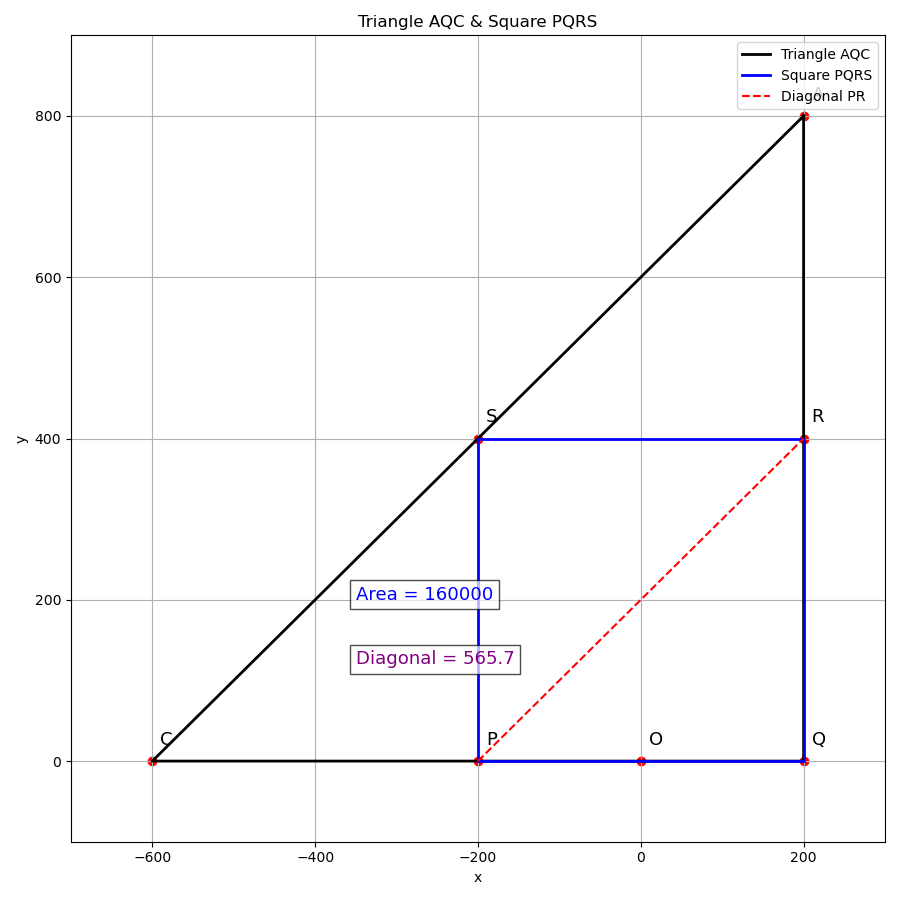
\includegraphics[width=0.8\linewidth]{figs/fig1.png}
            \caption{Plot of the square and triangle}
            \label{fig1}
        \end{figure}
\end{document}
